%%% Класс документа
\documentclass[a4paper,14pt]{article}

%%% Работа с русским языком
\usepackage{cmap}					% поиск в PDF
\usepackage[warn]{mathtext}
\usepackage[T2A]{fontenc}			% кодировка
\usepackage[utf8]{inputenc}			% кодировка исходного текста
\usepackage[english,russian]{babel}	% локализация и переносы
\usepackage{mathtext} 				% русские буквы в формулах
\usepackage{csvsimple}              % for tabular from csv loading
\usepackage{indentfirst}            % indent after sections
%\usepackage{minipage}

%%% Дополнительная работа с математикой
\usepackage{amsmath,amsfonts,amssymb,amsthm,mathtools} % AMS
\usepackage{icomma} % "Умная" запятая: $0,2$ --- число, $0, 2$ --- перечисление

%%% Номера формул
%\mathtoolsset{showonlyrefs=true} % Показывать номера только у тех формул, на которые есть \eqref{} в тексте.
%\usepackage{leqno} % Немуреация формул слева

%%% Шрифты
\usepackage{euscript}	 % Шрифт Евклид
\usepackage{mathrsfs}    % Красивый матшрифт

%%% Свои команды
\DeclareMathOperator{\sgn}{\mathop{sgn}}

%%% Перенос знаков в формулах (по Львовскому)
\newcommand*{\hm}[1]{#1\nobreak\discretionary{}
{\hbox{$\mathsurround=0pt #1$}}{}}

%%% Работа с картинками
\usepackage{graphicx}  % Для вставки рисунков
\graphicspath{{images/}{images2/}}  % папки с картинками
\setlength\fboxsep{3pt} % Отступ рамки \fbox{} от рисунка
\setlength\fboxrule{1pt} % Толщина линий рамки \fbox{}
\usepackage{wrapfig} % Обтекание рисунков и таблиц текстом

%%% Работа с таблицами
\usepackage{array,tabularx,tabulary,booktabs} % Дополнительная работа с таблицами
\usepackage{longtable}  % Длинные таблицы
\usepackage{multirow} % Слияние строк в таблице

%%% Теоремы
\theoremstyle{plain} % Это стиль по умолчанию, его можно не переопределять.
%\newtheorem{theorem}{Теорема}[section]
%\newtheorem{proposition}[theorem]{Утверждение}
 
%\theoremstyle{definition} % "Определение"
%\newtheorem{corollary}{Следствие}[theorem]
%\newtheorem{problem}{Задача}[section]
 
%\theoremstyle{remark} % "Примечание"
%\newtheorem*{nonum}{Решение}

%%% Программирование
\usepackage{etoolbox} % логические операторы

%%% Страница
\usepackage{extsizes} % Возможность сделать 14-й шрифт
\usepackage{geometry} % Простой способ задавать поля
	\geometry{top=25mm}
	\geometry{bottom=35mm}
	\geometry{left=35mm}
	\geometry{right=20mm}
	
%%% Колонтитулы
%\usepackage{fancyhdr}
 	%\pagestyle{fancy}
 	%\renewcommand{\headrulewidth}{0mm}  % Толщина линейки, отчеркивающей верхний колонтитул
 	%\lfoot{Нижний левый}
 	%\rfoot{Нижний правый}
 	%\rhead{Верхний правый}
 	%\chead{Верхний в центре}
 	%\lhead{Верхний левый}
 	% \cfoot{Нижний в центре} % По умолчанию здесь номер страницы
 	
%%% Интерлиньяж
%\usepackage{setspace}
%\onehalfspacing % Интерлиньяж 1.5
%\doublespacing % Интерлиньяж 2
%\singlespacing % Интерлиньяж 1

%%% Гиперссылки
\usepackage{hyperref}
\usepackage[usenames,dvipsnames,svgnames,table,rgb]{xcolor}
\hypersetup{				% Гиперссылки
    unicode=true,           % русские буквы в раздела PDF
    pdftitle={Заголовок},   % Заголовок
    pdfauthor={Автор},      % Автор
    pdfsubject={Тема},      % Тема
    pdfcreator={Создатель}, % Создатель
    pdfproducer={Производитель}, % Производитель
    pdfkeywords={keyword1} {key2} {key3}, % Ключевые слова
    colorlinks=true,       	% false: ссылки в рамках; true: цветные ссылки
    linkcolor=red,          % внутренние ссылки
    citecolor=green,        % на библиографию
    filecolor=magenta,      % на файлы
    urlcolor=cyan           % на URL
}

%%% Другие пакеты
\usepackage{lastpage} % Узнать, сколько всего страниц в документе.
\usepackage{soul} % Модификаторы начертания
\usepackage{csquotes} % Еще инструменты для ссылок
%\usepackage[style=authoryear,maxcitenames=2,backend=biber,sorting=nty]{biblatex}
\usepackage{multicol} % Несколько колонок
\usepackage{multirow} % Несколько строк

%%% Шрифты
%\renewcommand{\familydefault}{\sfdefault} % Начертание шрифта


%%% Работа с библиографией
%\usepackage{cite} % Работа с библиографией
%\usepackage[superscript]{cite} % Ссылки в верхних индексах
%\usepackage[nocompress]{cite} % 
%\usepackage{csquotes} % Еще инструменты для ссылок


%%% Tikz
\usepackage{tikz} % Работа с графикой
\usepackage{pgfplots} % Работа с pgf
\usepackage{pgfplotstable}
\usepackage{upgreek}

%%% Дополнительные пакеты для tikz
%\usepgfplotslibrary{dateplot} % Возможность подписания дат
\pgfplotsset{compat=1.5}

\author{Филиппенко Павел, Сибгатуллин Булат}
\title{Верстка научных отчетов в \LaTeX{}}
\date{\today}

\begin{document}    
    %% сделать красивый титульник
    \maketitle
    \thispagestyle{empty}

    \newpage
    \tableofcontents{} %содержание
    \newpage

    \section{\LaTeX{} что это такое?}

    \subsection{Введение}

    Любую лабораторную работу или научную статью важно не только сделать правильно и грамотно, но и добиться того, чтобы она была презентабильной и хорошо выглядела. В этом нам поможет культовая среда для верстки \LaTeX{}.
    %% вставить эмблему латеха
    Для оформления лабораторных работ или иных документов многие используют Word или LibreOffice Writer. Однако обе эти программы имеют ряд недостатков и в вопросе верстки научного текста значительно уступают \LaTeX{}.

    Что такое \LaTeX{}?  
    Согласно Википедии: \LaTeX{} -- наиболее популярный набор макрорасширений (или макропакет) системы компьютерной вёрстки \TeX, который облегчает набор сложных документов. Пакет позволяет автоматизировать многие задачи набора текста и подготовки статей, включая набор текста на нескольких языках, нумерацию разделов и формул, перекрёстные ссылки, размещение иллюстраций и таблиц на странице, ведение библиографии и др.
    Возможно данное определение звучит несколько сложновато. Не забивая голову лишним, можете считать \LaTeX инструментом оформления научных отчетов. Более глубокое понимание придет с практикой.

    \begin{figure}[h!]
        \centering
        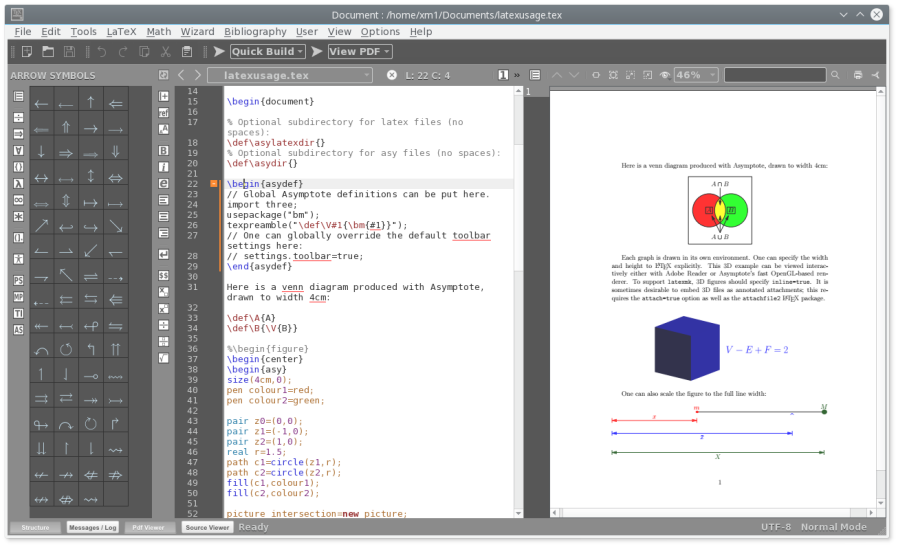
\includegraphics[width = \textwidth]{TexCode_example.png}
        \caption{}
        % \label{}
    \end{figure}

    \newpage

    \subsection{Преимущества \LaTeX}

    Чем же так хорош \LaTeX? В целом можно выделить 4 основных преимущества

    \begin{enumerate}
        \item Подгоняет документ ко всем типографским стандартам. Таким образом, можно полностю сконцентрироваться на содержании документа, а не на его оформлении.
        \item Автоматизация процессов: автоматическая нумерация разделов и формул, автоматическое составление оглавления и многое другое. Меньше рутины.
        \item Открытая среда. Обширное community. В интернете можно найти ответы на любые ваши вопросы, большое количество информации, а так же пакетов, расширений и фич.
        \item Кроссплатформенность.
    \end{enumerate}

    \subsection{Как оно работает???}

    В некотором смысле работа LaTeX похож на известные вам языки программирования. На вход подается исходный код, затем происходит компиляция и на выходе мы получаем тепленький красивый pdf-документ.

    %% картинки исходного кода и готового документа

    \section{Редакторы кода}

    Для работы с \LaTeX необходимо 2 вещи: специальный компилятор, который будет магическим образом превращать ваши исходники в pfd и редактор кода, в котором вы будете непосредственно работать.
    
    \begin{wrapfigure}{l}{0.25\textwidth}
        \centering
        
\includegraphics[width = 0.2\textwidth]{texmaker220-220.jpg}
        \caption{}
        %\label{fig:}
    \end{wrapfigure}

    Существует большое количество программ, которые представляют собой визуальную графическую среду для создания и редактирования документов \LaTeX.
    Наиболее распространенным вариантом являются программы TexMaker и TexStudio. Это кросс-платформенные редакторы \LaTeX с открытым кодом. Данные программы являются интегрированными средами для создания \LaTeX документов и включают такие возможности, как интерактивная система проверки правописания, сворачивание блоков текста, подсветка синтаксиса и многое другое.

    \begin{wrapfigure}{r}{0.25\textwidth}
        \centering
        
\includegraphics[width = 0.2\textwidth]{Texstudio_Logo.png}
        \caption{}
        %\label{fig:}
    \end{wrapfigure}

    % фотографи TexMaker и TexStudio

    %% Пара слов про VS-Code

    Мы же будем использовать веб-редактор латех документов OverLeaf. Его основное преимущество заключается в том, что данный редактор не требует никакой установки, воспользоваться им можно с любой платформы на любом устройстве с выходом в интернет.
    Кроме того, этот редактор позволяет нескольким пользователям редактировать один и тот же документ одновременно и просматривать изменения друг друга в режиме реального времени.

    \begin{figure}[h!]
        \centering
        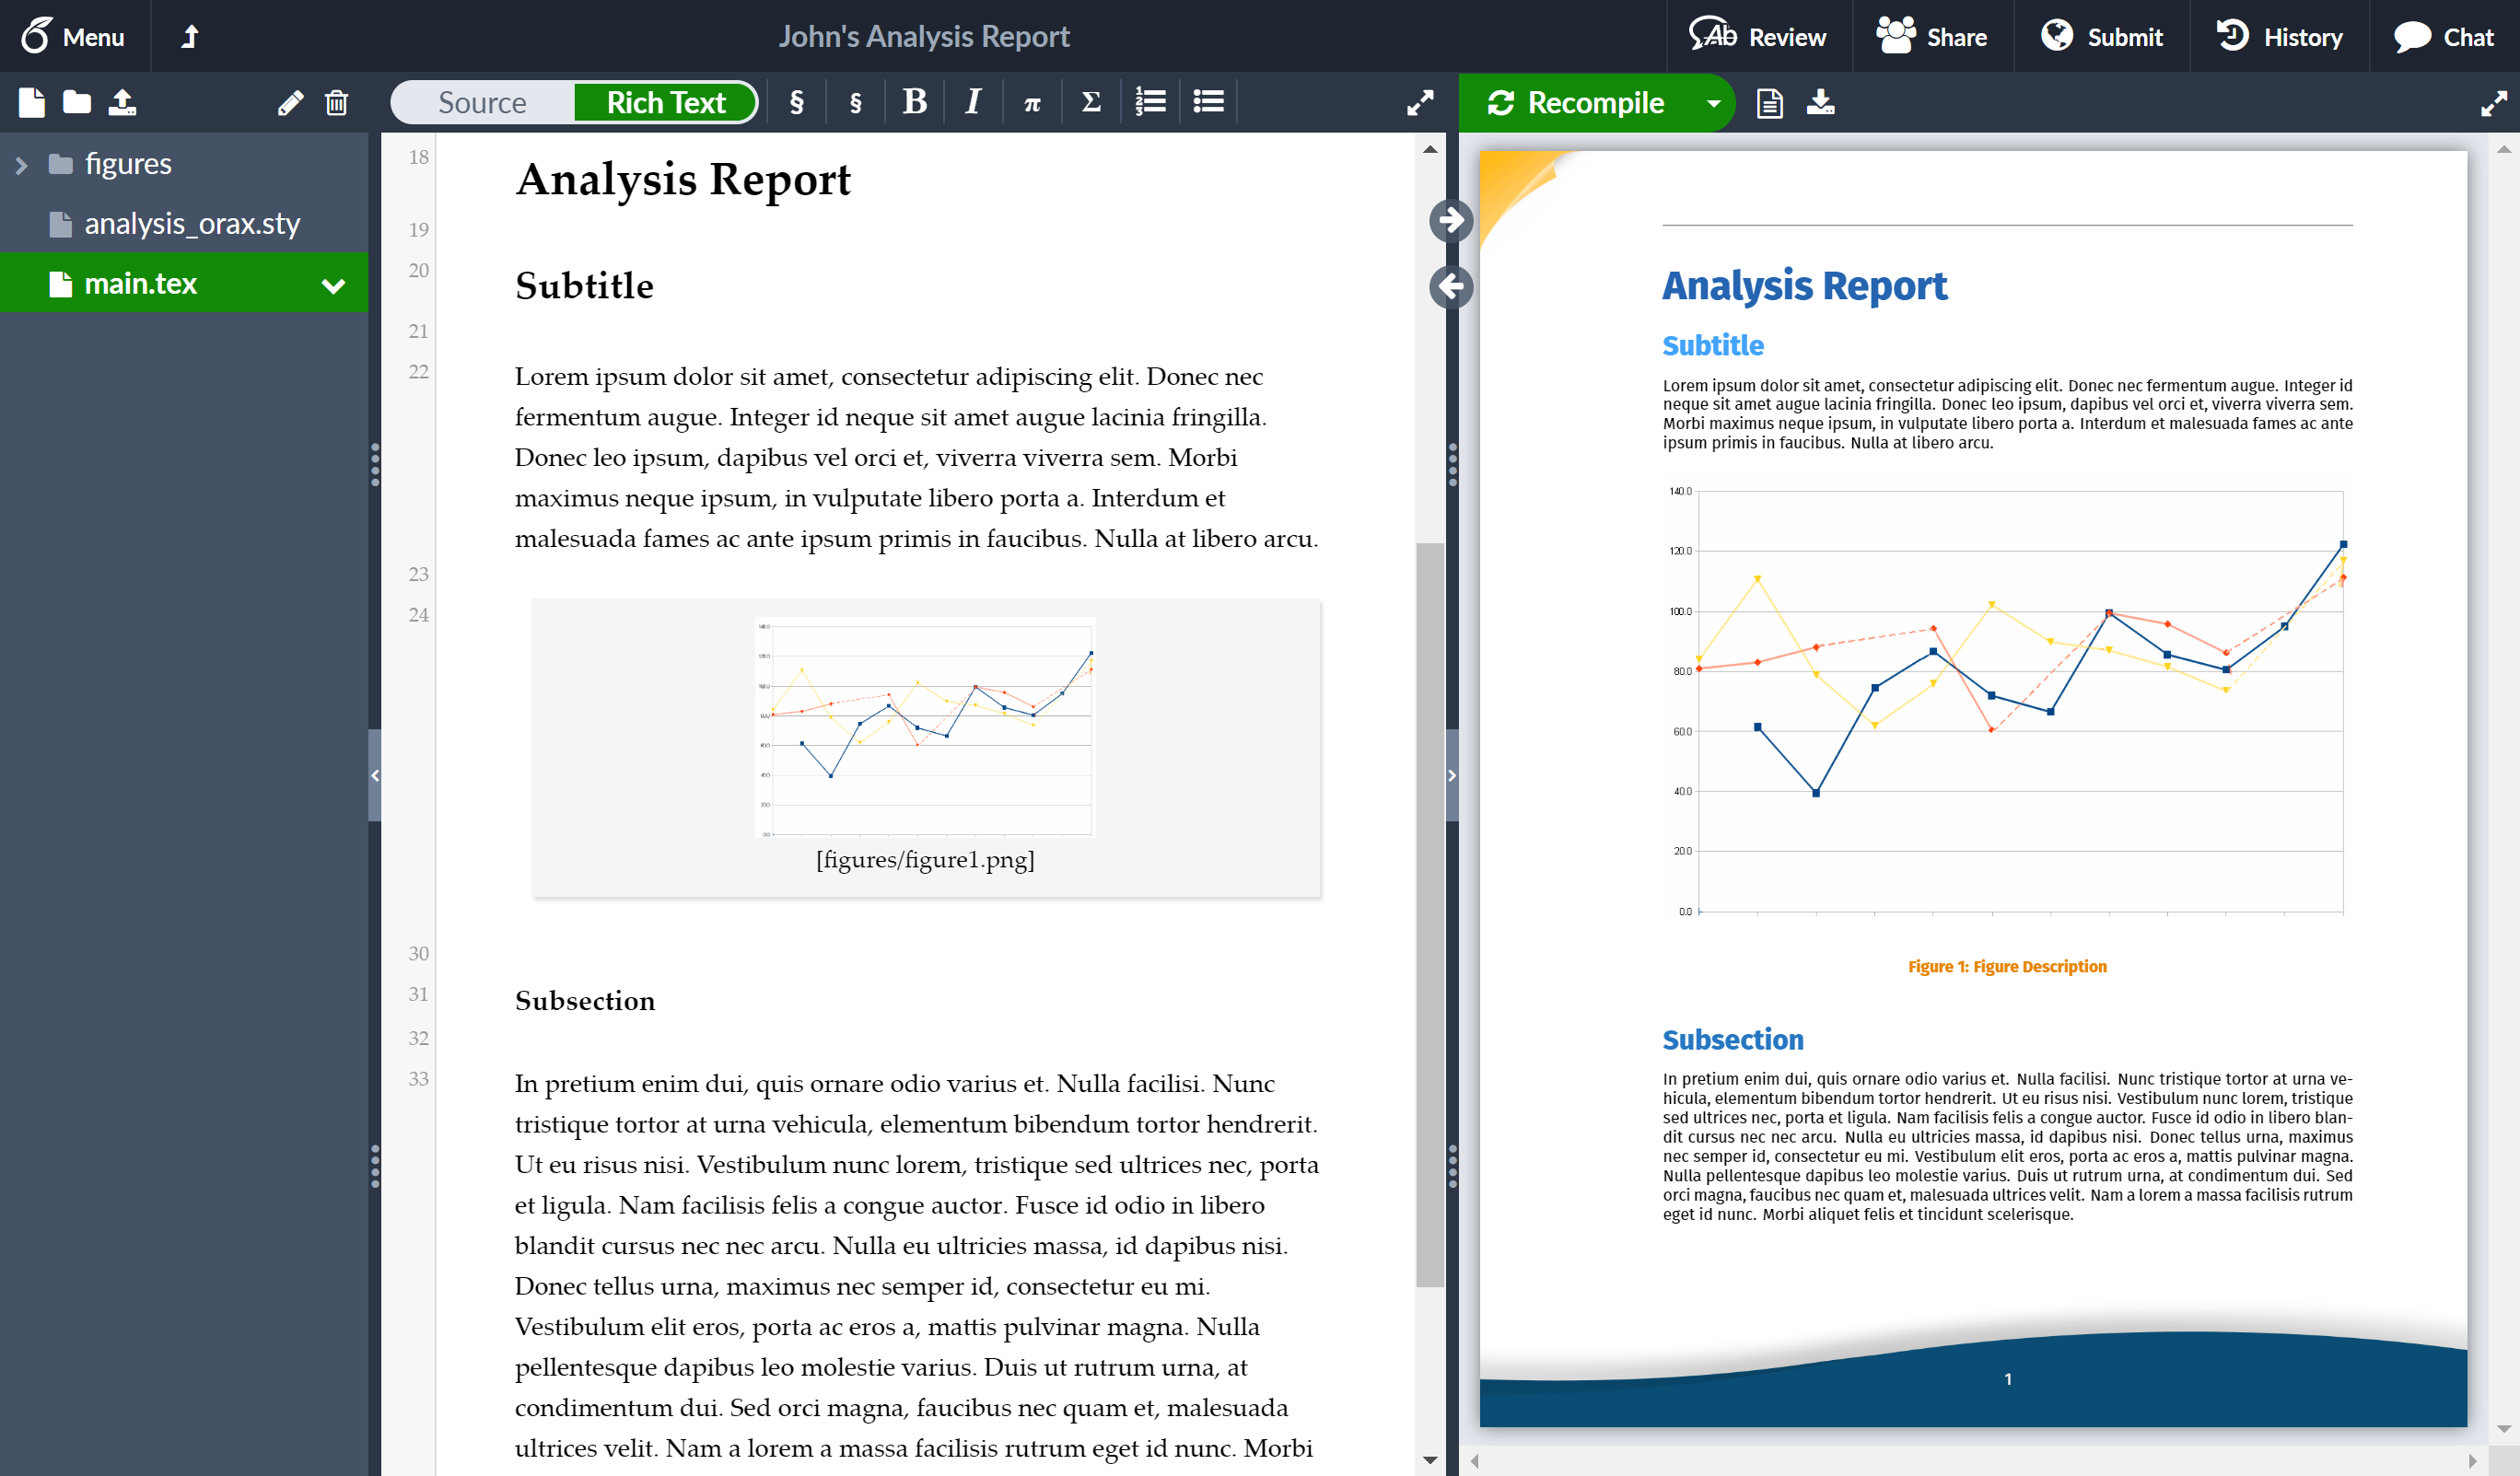
\includegraphics[width=\linewidth]{OverLeaf_example.png}
        \caption{}
        \label{OverLeaf_example}
    \end{figure}

    \section{Overleaf}

    \subsection{Регистрация}

    Давайте же познакомимся с нашим текстовым редактором. Для этого перейдем на сайт 
    \href{https://www.overleaf.com/login}{https://www.overleaf.com/login} 
    % https://www.overleaf.com/login 
    и сразу попадем на страницу регистрации. 

    %% input a beautiful instruction pictures
    
    Чтобы зарегистрироваться, необходимо внизу экрана выбрать пункт Register.

    %% input a beautiful instruction pictures

    Вводим адрес электронной почты и придумываем пароль. После этого на вам предложат создать ваш первый проект, а на почту придет письмо с просьбой подтвердить адрес. Абсолютно ничего сложного,
    подтверждаем адрес и создаем наш первый проект Blank Project.

    %% input a beautiful instruction pictures

    \subsection{Знакомство с интерфейсом}

    После того, как вы создали ваш первый в жизни tex-project вас перенесет в рабочее пространство OverLeaf. Здесь будет
    проходить большая часть вашей работы.

    \begin{figure}[h!]
        \centering
        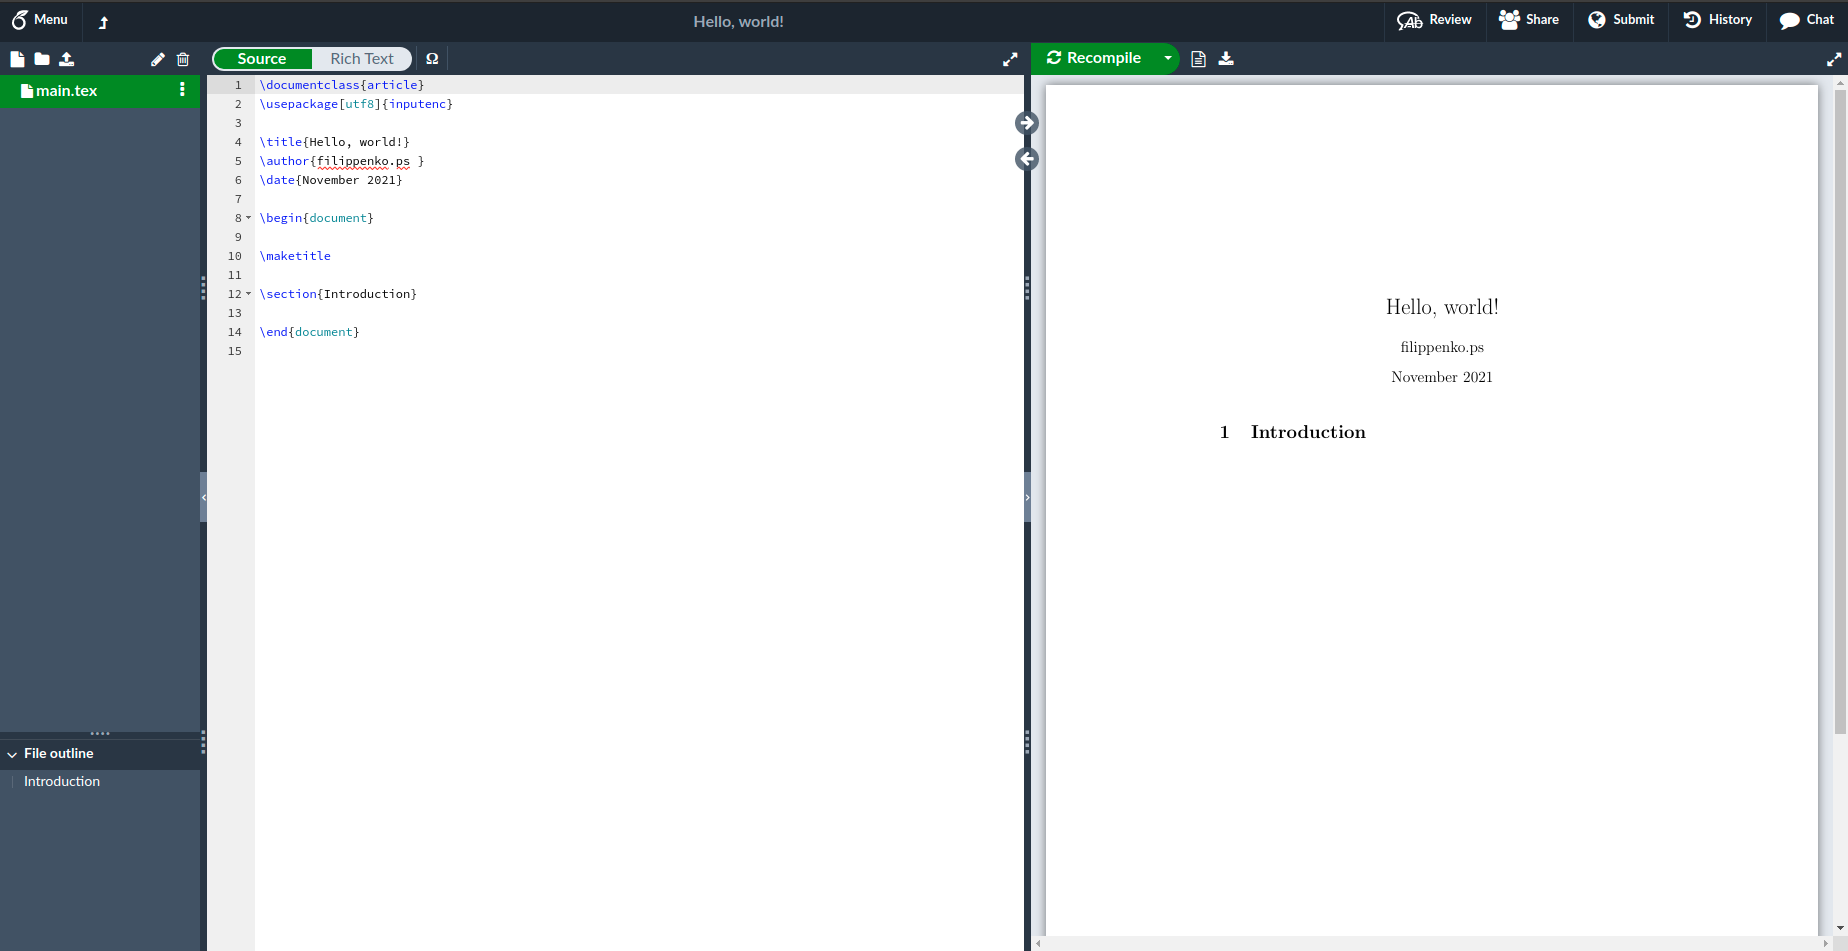
\includegraphics[width = \textwidth]{OverLeafWorkingSpace.png}
        \caption{}
        % \label{}
    \end{figure}

    Все пространство можно условно разделить на 3 главные смысловые области. 
    
    Первая область -- рабочая, здесь вы будете писать
    теховский код, который потом отправится на обработку компилятору. 
    
    Вторая область -- область визуализации, здесь вы
    можете посмотреть текущий вид вашего pdf-документа. 
    
    Третья область -- вспомогательная, в этой области вы можете видеть
    все файлы и папки вашего текущего проекта, а так же мини-оглавление вашей работы.

    %% вставить поясняющие картинки, цветом выделить обозначенные области

    Нажав на кнопочку <<Menu>> на верхней панели слева, вам откроется меню детальной настройки документа (что-то страшное, трогать пока не будем).
    А нажав на стрелочку рядом, мы выйдем в главное меню управления проектами.

    \begin{figure}[h!]
        \centering
        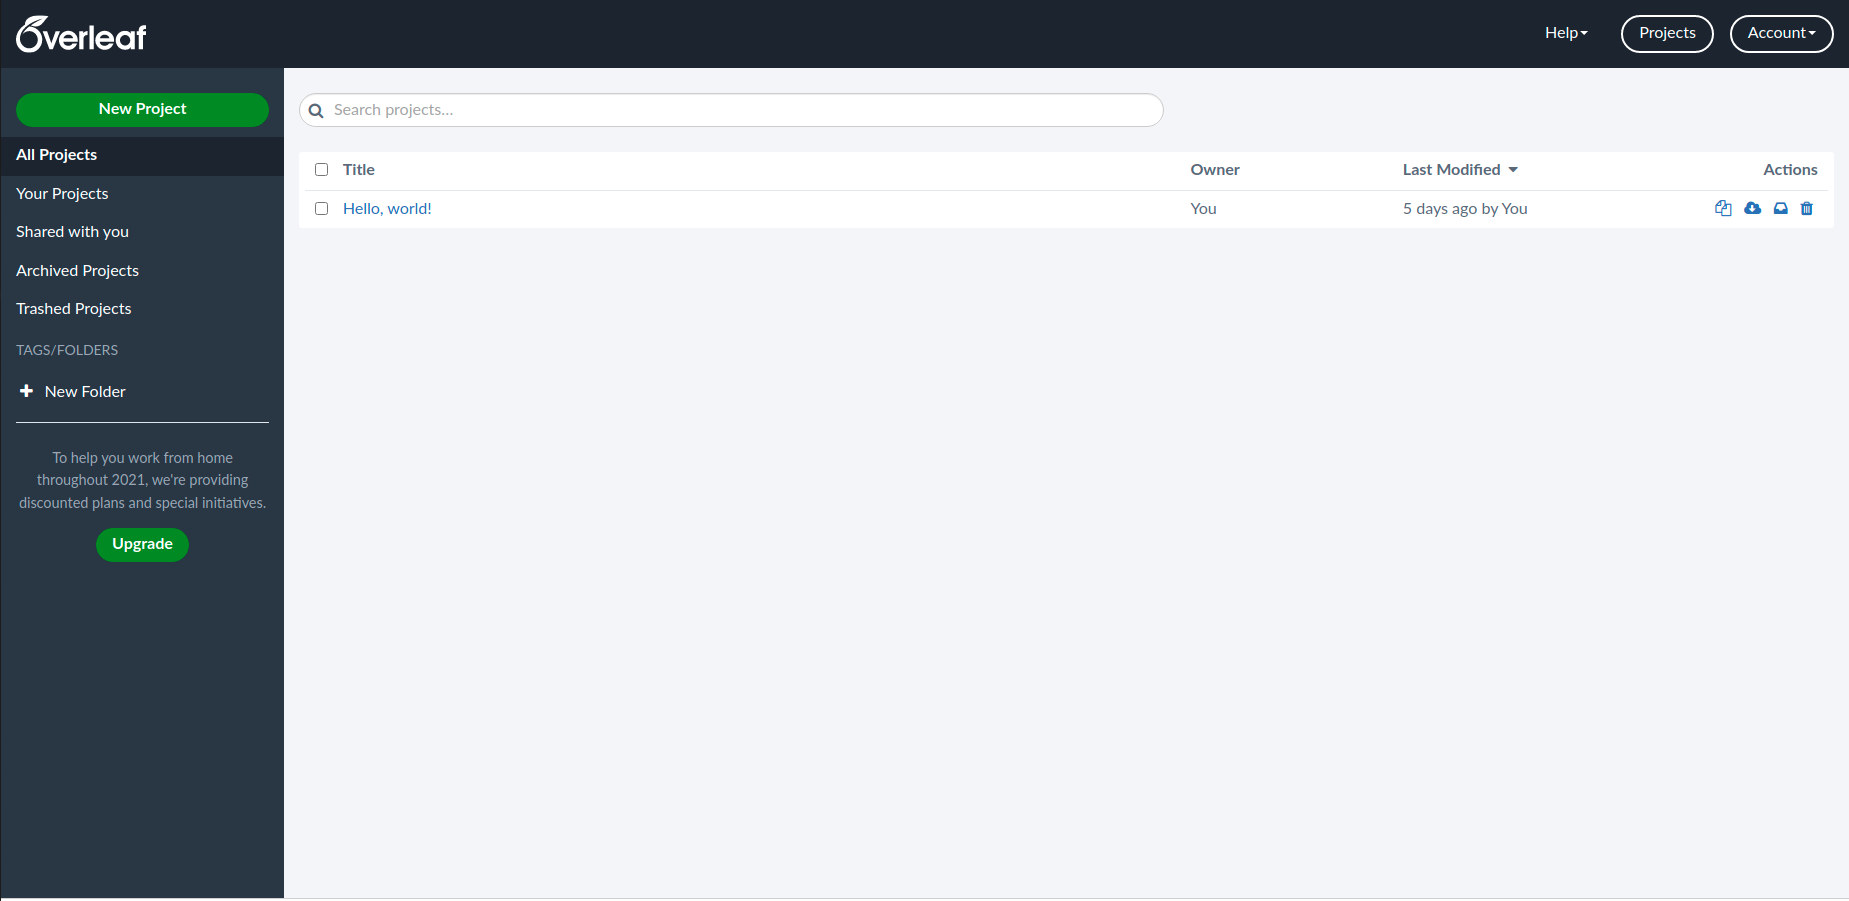
\includegraphics[width = \textwidth]{projects_manage_space.png}
        \caption{}
        % \label{}
    \end{figure}

    В этом меню вам доступно управление вашим аккаунтом, а так же управление всеми вашими латеховскими проектами проектами.

    \section{Начало работы}

    Наконец, мы приступаем к написанию нашего документа. Перейдем в наш <<проект Hello world!>> и в рабочей области удалим весь сгенерированный по умолчанию код.

    Перед тем, как наполнять наш документ содержанием и смыслом, необходимо настроить его вид и подключить используемые пакеты.

    %% временное решение для оформления исходноо кода
    %  окружение запрещает теху обрабатывать все, что находится внутри
    \begin{verbatim}
        \documentclass[a4paper,12pt]{article}

        % Русский язык
        \usepackage[T2A]{fontenc}
        \usepackage[utf8]{inputenc}	
        \usepackage[english,russian]{babel}

        % Математика
        \usepackage{amsmath,amsfonts,amssymb,amsthm,mathtools} 
    \end{verbatim}

    Первой командой мы требуем, чтобы \LaTeX{} сгенерировал наш документ типа article (статья) на бумаге размера A4, со стандартным шрифтом размера 12.
    Следующие 3 строчки подключают пакеты для работы с русским языком, а самая последняя строчка подключает математические пакеты.
    Кстати, как вы могли заметить, значком \% обозначаются комментарии. Комментарии помогут вам легче ориентироваться в вашем коде,
    все что начинается со значка \% будет игнорироваться компилятором.
    
    Итак, мы подключили базовые пакеты, без которых невозможна работа в латех. Далее мы подключим еще
    несколько пакетов, которые понадобятся нам в дальнейшем, а затем перейдем к написанию статьи.

    \begin{verbatim}
        \usepackage{graphicx}  % импорт изображений
        \graphicspath{images/} % папка с картинками
        \usepackage{caption}

        % центрирование подписи к картинке
        \captionsetup{justification=centering}

        \usepackage{hyperref}  % работа с сылками

        % настроим поля и колонтинулы страницы
        \usepackage{geometry} %
            \geometry{top=25mm}
            \geometry{bottom=35mm}
            \geometry{left=35mm}
            \geometry{right=20mm}
    \end{verbatim}

    Подготовительная работа закончена и мы можем приступить к написанию документа.

    %Добавить раздел работа с текстом, в нем описать нужные термины

    \section{Работа с текстом}

    Наш основной код начинается с окружения
    
    \begin{verbatim}
        \begin{document} % начало документа
        \end{document} % конец документа
    \end{verbatim}

    эти строчки обозначают соответственно начало и конец нашего основного документа, именно внутри этого окружения мы будем писать наш основной контент.

    Теперь займемся смысловым наполнением нашего документа. Межу 
    командами begin и end напишем нашу первую строчку:

    \begin{verbatim}
        \begin{document} % начало документа
        Наша первая строчка.
        \end{document} % конец документа
    \end{verbatim}
    Для того, чтобы скомпилировать полученный код, нажмем сочетание
    клавиш \textbf{Ctrl + S}, или зеленую кнопочку \textbf{Recompile} на страничке редактора Overleaf.

    В области визуализации pdf-документа можем убедиться, что написанная нами строчка появилась в нашем будущем документе.

    Попробуем написать вторую строчку под первой, а затем, заново
    скомпилировать документ. Здесь мы сталкиваемся с первой проблемой:
    вопреки нашему желанию вторая строчка напечаталась рядом с первой, а не под ней, 
    так, как это было в исходнике.\\[1 cm] 

    \begin{minipage}[h!]{0.5\linewidth}
    \begin{verbatim}
    \begin{document}
    Наша первая строчка.
    Вторая строчка.
    \end{document}
    \end{verbatim}
    \end{minipage}
    \hfill
    \begin{minipage}[h!]{0.5\linewidth}
    Наша первая строчка.
    Вторая строчка
    \end{minipage}

    Для того, чтобы перейти на новую строку в \LaTeX есть несколько способов

    \begin{enumerate}
        \item Если вы хотите начать новый абзац, то нужно оставить одну пустую строку.

    \begin{minipage}[h!]{0.5\linewidth}
    \begin{verbatim}
    \begin{document}
    Наша первая строчка.

    Вторая строчка.
    \end{document}
    \end{verbatim}
    \end{minipage}
    \hfill
    \begin{minipage}[h!]{0.5\linewidth}
    Наша первая строчка.

    Вторая строчка
    \end{minipage}

    \item Если вы хотите просто перенести текст на следующую строчку, не начиная при этом новый абзац, То
    в конце строки необходимо поставить $\backslash \backslash$.

    \begin{minipage}[h!]{0.5\linewidth}
    \begin{verbatim}
    \begin{document}
    Наша первая строчка.\\
    Вторая строчка.
    \end{document}
    \end{verbatim}
    \end{minipage}
    \hfill
    \begin{minipage}[h!]{0.5\linewidth}
    Наша первая строчка.\\
    Вторая строчка
    \end{minipage}

    \item Если вы ходите получить вертикальный отступ, какого-то фиксированного размера,
    вы можете указать этот размер в квадратных скобках, после $\backslash \backslash$.

\begin{minipage}[h!]{0.5\linewidth}
\begin{verbatim}
\begin{document}
Наша первая строчка.\\[1 cm]
Вторая строчка.
\end{document}
\end{verbatim}
\end{minipage}
\hfill
\begin{minipage}[h!]{0.5\linewidth}
Наша первая строчка.\\[1 cm]
Вторая строчка
\end{minipage}

    \end{enumerate}

    Похожая ситуация в \LaTeX и с горизонтальными пробелами.
    Если между двумя словами, вы поставите 5 пробелов, в конечном
    документе, между этими словами все равно будет один пробел.\\[0.5 cm]
    
\begin{minipage}[h!]{0.5\linewidth}
\begin{verbatim}
\begin{document}
The first     the second.
\end{document}
\end{verbatim}
\end{minipage}
\hfill
\begin{minipage}[h!]{0.5\linewidth}
    The first     the second.
\end{minipage} \\[0.5 cm]

    Для того, чтобы сделать горизонтальный отступ заданного размера,
    применим команду $\backslash hspace\{\}$ \\[5 mm]

\begin{minipage}[h!]{0.5\linewidth}
\begin{verbatim}
\begin{document}
The first \hspace{5 mm} 
the second.
\end{document}
\end{verbatim}
\end{minipage}
\hfill
\begin{minipage}[h!]{0.5\linewidth}
The first \hspace{5 mm} the second.
\end{minipage} \\[5 mm]

    Приведем в табличке некоторые команды офорлмения текста, поэксперементировать с ними вы можете самомтоятельно.

    \begin{center}
        \begin{tabular}{|c|c|c|}
            \hline
            Стиль оформления & команда & результат\\
            \hline
            \hline
            Выделить жирным & $\backslash textbf\{\}$ & \textbf{text} \\
            \hline
            Выделить курсивом & $\backslash textit\{\}$ & \textit{text} \\
            \hline
            Подчеркнуть & $\backslash underline\{\}$ & \underline{text} \\
            \hline
            Взять в рамочку & $\backslash fbox\{\}$ & \fbox{text} \\
            \hline
        \end{tabular}
    \end{center}

    Закончить раздел работы с текстом, мне бы хотелось кратким описанием разделов документа.
    \LaTeX предлогает удобную иерархию создания разделов, подразделов, подпод разделов и так далее.
    
    Для того, чтобы создать в документе новый раздел необходимо воспользоваться
    командой $\backslash section\{\}$, подраздел $\backslash subsection\{\}$,
    ну а подподраздел $\backslash section\{\}$. В фигурных скобочках пишется названия раздела,
    причем, \LaTeX автоматически нумерует его. При этом, если вы хотите создать ненумерованный
    раздел или подраздел, необходимо поставить символ * после слова section.

    \begin{center}
        \begin{verbatim}
            \section*{SctionName}
        \end{verbatim}
    \end{center}

    \section{Математика}

    Теперь, когда вы умеете работать с текстом вам нужно понять, как в \LaTeX{} записываются и оформляются математический выражения. Для выделения формул в \LaTeX{} используются две конструкции. Если получившиеся выражение вам важно и вы хотите его отметить (чтобы использовать в дальнейшем или по другой причине), то вам нужно использовать такую запись:

    \begin{equation}
        y = f(x)
    \end{equation}
    
    Вот так будет выглядеть ее код:    
    
    \begin{verbatim}
        \begin{equation}
            y = f(x)
        \end{equation}
    \end{verbatim}   
    
    Видно, что данное выражение обрамлено в $\backslash begin\{equation\}$ ... $\backslash end\{equation\}$, так компилятор понимает, что мы будем записывать математические символы. Заметьте, что при такой форме записи \LaTeX{} самостоятельно записывает номер данного выражения, а следовательно, если вы хотите обратиться к какой-то формуле, уже записанной у вас в документе, вы можете просто записать её номер.
    
    В случае если ваша выражение является результатом промежуточных вычислений и не будет использоваться в дальнейшем, то стоит показать это при помощи второго вида записи:
    
    $$y = f(x)$$    
    
    И сделать это можно при помощи \$\$:    
    
    \begin{verbatim}
        $$y = f(x)$$
    \end{verbatim}
    
    Также, если вы хотите использовать в тексте какое-либо математическое выражение вам нужно выделить его \$ (теперь только одним):

    Some text: $e^x$. И вот так это выглядит в коде:
    
    \begin{verbatim}
        Some text: $e^x$
    \end{verbatim}
    
    Теперь посмотрим, как в \LaTeX{} будут записываться некоторые математические символы:
    
    $$e^x, e^{abc}, e^abc$$
        
    $$e_x, e_{abc}, e_abc$$
    
    $$e^{xyz}_{abc}$$
    
    \begin{verbatim}
        $$e^x, e^{abc}б e^abc$$
        
        $$e_x, e_{abc}, e_abc$$
        
        $$e^{xyz}_{abc}$$
    \end{verbatim} 
    
    Здесь вы можете видеть, как в \LaTeX{} записывается степень и индекс, а также из комбинация. Также обратите внимание на то, что если в степени или индексе больше одного символа, то их нужно брать в фигурные скобки.
    
    Часто бывает нужно (при использовании знака суммы или интеграла), чтобы степень и индекс перешли в пределы (например суммирования или интегрирования). Сделать это мы можем при помощи выражения $\backslash$limits, записанного после нужного нам символа, но перед его степенью и индексом:
    
    $$\int\limits^{x_{\text{макс}}}_{0}$$
    
    \begin{verbatim}
        $$\int\limits^{x_{\text{макс}}}_{0}$$
    \end{verbatim}
    
    Обратите внимание, что здесь мы использовали русский текст в записи выражения. Для его использования вам нужно будет написать $\backslash text\{\}$ и текст в фигурных скобках. При использовании английского языка можно просто писать на нем без использования $\backslash text\{\}$.
    
    Стоит отметить, что в \LaTeX{} часто приходится использовать формулы раной "высоты", поэтому здесь есть выражения для подгона высоты скобок под высоту формулы. Посмотрите как она реализована на примере обычной дроби:
    
    $$\left( \frac{x}{y} \right) $$
    
    \begin{verbatim}
        $$\left( \frac{x}{y} \right) $$
    \end{verbatim}
    
    Дробь здесь была задана выражением $\backslash frac\{\}\{\}$ (в первой скобке записывается числитель, а во второй знаменатель. За подгон высоты скобок к высоте выражения отвечают надписи $\backslash$right и $\backslash$left перед скобками. Их вы можете использовать с люьым видом скобок (фигурными, прямоугольными и т.д.).
    
    
    
    На этом блок посвященный математике подходит к концу, и еси вы ожидали увидеть тут разбор существующи в \LaTeX{} символов, то мне стоит вас огорчить, так как этого тут не будет. Использование символов сводится к простому поиску кода символа и не представляетс из себя ничего сложного. Сложности обычно вызывают использование символов одновременно со степенями, дробями (в первую очередь из-за скобок), а это мы уже с вами разобрали.
    
    \section{Рисунки и таблицы}

    В составлении отчета важное место занимают различные таблицы с данными, графики, схемы установок и другие таблицы и рисунки, поэтому в \LaTeX{} реализована работа как с таблицами, так и со вставкой изображений. Для начала рассмотрим изображения:
    
    \begin{figure}[h!]
        \centering
        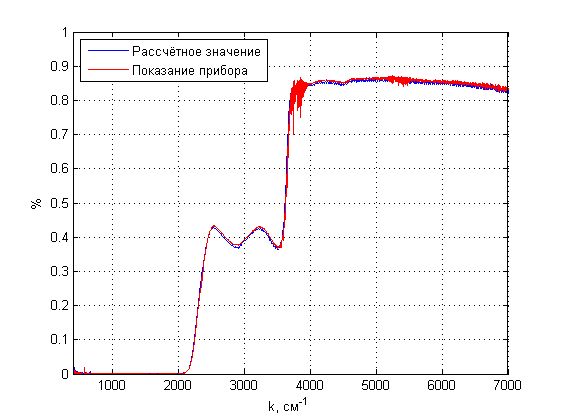
\includegraphics[width=0.5\linewidth]{9.png}
        \caption{Коэффициент пропускания стекла}
    \end{figure}
    
    Вот как выглядит код для такого изображения:
    
    \begin{verbatim}
        \begin{figure}[h!]
            \centering
            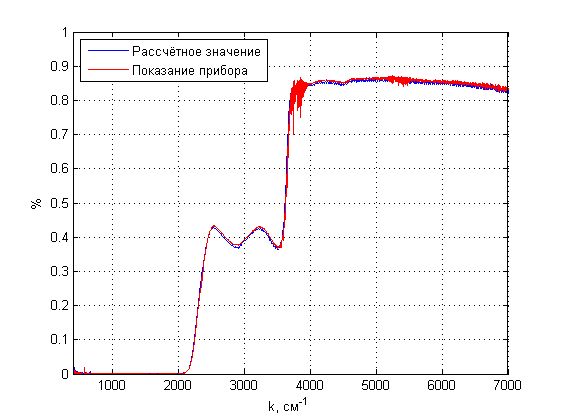
\includegraphics[width=0.5\linewidth]{9.png}
            \caption{Коэффициент пропускания стекла}
        \end{figure}
    \end{verbatim}
    
    Посмотрим, что происходит в данном фрагменте хода. Все функции обрамлены $\backslash begin\{figure\}[h!]$ ... $\backslash end\{figure\}$, так компилятор понимает, что здесь мы будем вставлять изображение, h! в квадратных скобках означает, что изображение должно стоять в первом подходящем месте. Подключение изображения реализуется функцией $\backslash includegraphics[]\{\}$ в квадратных скобках при помощи width прописывается длина изображения по горизонтали. Ее можно задать например при помощи $*\backslash linewidth$, где $\backslash linewidth$ - горизонтальный размер страницы с учетом отступов, а * - число, на которое длина этой строки будет умножаться в нашем случае оно равно 0.5, а значит что изображение будет занимать только половину страницы. Имя изображения записывается в фигурных скобках ($\{9.png\}$), про папку из которой берутся изображение мы говорили вначале методички, если такая папка не задана, то по умолчанию используется папка, в которой хранится файл с кодом.
    
    При помощи $\backslash caption\{\}$ мы задаем описание к изображению, причем номер рисунка перед ним прописывается автоматически. $\backslash centering$ распологает изображение и все его дополнительные свойства по центру (в нашем случае описание).
    
    Если вам нужно расположить рядом несколько графиков, то вы можете сделать расположив их в ряд в одной строке. Для этого можно использовать функцию minipage:
    
    \begin{figure}[h!]
        \begin{center}
            \begin{minipage}[h!]{0.48\linewidth}
                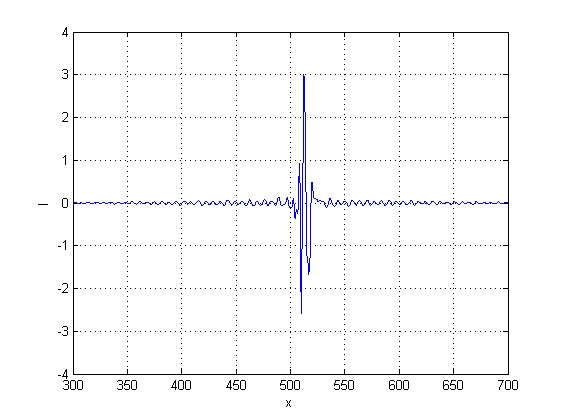
\includegraphics[width=1\linewidth]{2.png}
                \caption{Экспериментально полученная интерферограмма для пустого канала}
            \end{minipage}
            \hfill
            \begin{minipage}[h!]{0.48\linewidth}
                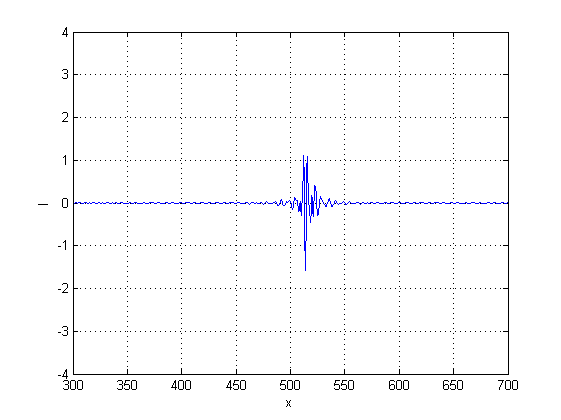
\includegraphics[width=1\linewidth]{3.png}
                \caption{Экспериментально полученная интерферограмма для стекла}
            \end{minipage}
        \end{center}
    \end{figure}
    
    Разберем код данного фрагмента:
    
    \begin{verbatim}
        \begin{figure}[h!]
            \begin{center}
                \begin{minipage}[h!]{0.48\linewidth}
                    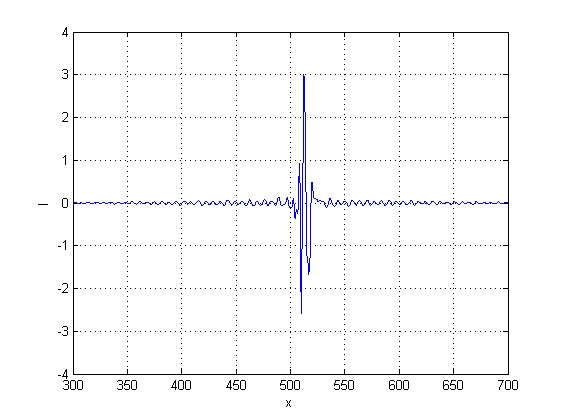
\includegraphics[width=1\linewidth]{2.png}
                    \caption{Экспериментально полученная
                     интерферограмма для пустого канала}
                \end{minipage}
                \hfill
                \begin{minipage}[h!]{0.48\linewidth}
                    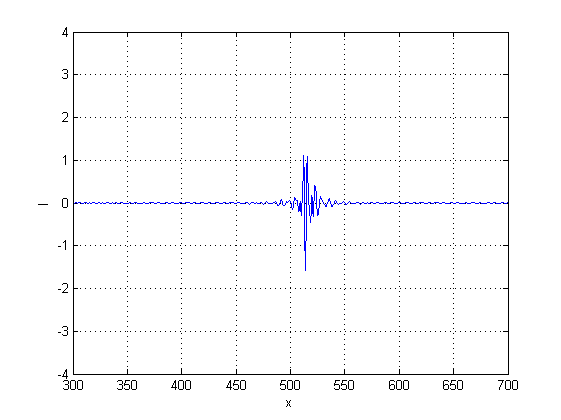
\includegraphics[width=1\linewidth]{3.png}
                    \caption{Экспериментально полученная
                     интерферограмма для стекла}
                \end{minipage}
            \end{center}
        \end{figure}
    \end{verbatim}
    
    В данном случае $\backslash centering$ нам будет недостаточно, так как он распологает по центру только изображение и все что с ним связано, а у нас используется два изображения. Поэтому вместо него мы используем знакомое нам выражение $\backslash begin\{center\}$ ... $\backslash end\{center\}$. Дальше мы используем $\backslash begin\{minipage\}[h!]\{0.48 \backslash linewidth\}$ ... $\backslash end\{minipage\}$. Как понятно из навзвания minipage означает маленькую страницу, горизонтальный размер которой задается уже аргументом во второй фигурной скобке. $\backslash hfill$ автоматически определяет нужно делать перенос строки или можно уместить изображение на этой же строчке. Также не ставьте значение горизонтального размера minipage равным 1 / (количество изображений на строку), так как между мини-страницами существует минимальное расстояние. Если вы ну будете учитывать его компилятор все еще сможете уместить все изображения в одну строку, но центрирование собьется.
    
    На этом мы заканчиваем работу с изображениями и переходим к таблицам. Вся работа с таблицами сводится к такому коду:
    
    \vspace{0.5cm}   
    
    \begin{center}    
        \begin{tabular}{|c|c|}
        \hline 
        Пример таблицы & Пример таблицы \\ 
        \hline 
        Пример таблицы & Пример таблицы \\ 
        \hline 
        \end{tabular}
    \end{center}
    
    \vspace{0.5cm}
    
    Ее код:    
    
    \begin{verbatim}
        \begin{center}
            \begin{tabular}{|c|c|}
            \hline 
            Пример таблицы & Пример таблицы \\ 
            \hline 
            Пример таблицы & Пример таблицы \\ 
            \hline 
            \end{tabular}
        \end{center}
    \end{verbatim}
    
    Таблица задается $\backslash begin\{tabular\}\{|c|c|\}$ ... $\backslash end\{tabular\}$. Здесь tabular дает компилятору понять, что мы имеем дело с таблицей. Символ \textit{c} в $\{|c|c|\}$ имеет смысл столбца, то есть каждая буква \textit{c} это один столбец. То, как столбцы разделяются задается символами | между буквами \textit{c}, их количество можно менять, либо вовсе убирать их. $\backslash hline$ - горизонтальная линия, разделяющая строки таблицы (их количество также можно менять, либо вовсе убирать их). Информация о переходе строки передается компилятору при помощи $\backslash \backslash$, а о следующем стоблце при помощи $\&$. Учитывайте, что если в строке будет недостаточно $\&$ или в таблице будет недостаточно $\backslash \backslash$, то компилятор выдаст уведомление об ошибке.
    
    Кстати внутри таблицы можно использовать формулы, текст и вставлять изображения.
    
    \section{Ссылки}

    Ссылки в \LaTeX{} помогают не только переходить на различные сайты, но и могут направить на нужную страницу, формулу, изображение и любой набор символов. Мы уже сталкивались с таким видом ссылок (называемых гиперссылками) в начале, когда оформляли оглавление, рассмотрим как еще можно с ними работать.
    
    Ссылки на страницы редко когда используются, поэтому здесь будут рассмотрено подключение ссылок к изображениям и формулам. Посмотрим на данное изображение:

    \newpage    
    
    \begin{figure}[h!]
        \centering
        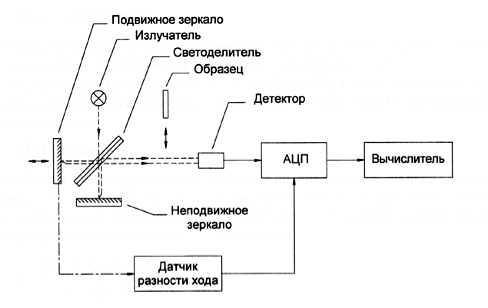
\includegraphics[width=0.48\linewidth]{1.png}
        \caption{Схема устройства Фурье-интерферометра}
        \label{picture}
    \end{figure}
    
    И его код:
    
    \begin{verbatim}
        \begin{figure}[h!]
            \centering
            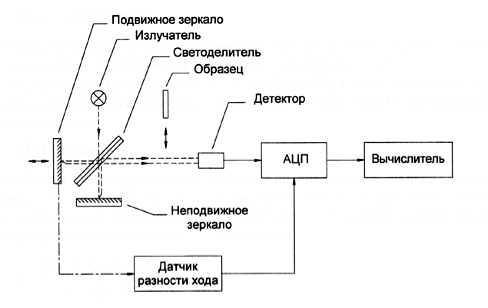
\includegraphics[width=0.48\linewidth]{1.png}
            \caption{Схема устройства Фурье-интерферометра}
            \label{picture_1}
        \end{figure}
    \end{verbatim}
    
    В коде появилось новое, незнакомое нам выражение: 

    \begin{verbatim}
        \label{picture_1}    
    \end{verbatim}

    $\backslash label\{\}$ задает метку, 
    с именем прописанным внутри фигурных скобок. На это имя теперь можно ссылаться, например так: $\ref{picture}$. Чтобы это сделать, нужно просто написать такой код:
    
    \begin{verbatim}
        $\ref{1}$
    \end{verbatim}
    
    Внутри фиурных скобок в данном выражении, вместо $picture\_1$ может быть имя любой другой метки. Кстати, хочу обратить ваше внимание, что $\backslash label\{\}$ должен идти после последней команды в обрамлении $\backslash begin\{figure\}[h!]$ ... $\backslash end\{figure\}$. Если данное условие выполнено не будет, то \LaTeX автоматически поменяют ссылку внутри $\backslash ref\{\}$ на ссылку на раздел, в котором находится данный код.
    
    При создании меток на формулу также используется $\backslash label\{\}$, но его расположение в коде отличается от такового у изображений:
    
    \begin{equation} \label{formula}
        \Delta I = I(x) - I(0)
    \end{equation}
    
    Код к $\eqref{formula}$:
    
    % \newpage
    
    \begin{verbatim}
        \begin{equation} \label{formula_1}
            \Delta I = I(x) - I(0)
        \end{equation}
    \end{verbatim}
    
    Заметьте, что у формул метка находится сразу после $\backslash begin\{equation\}$, так происходит потому что в обраблемнии для формулы обычно записывается только формула и больше ничего. Следовательно удобнее всего ставить метку на обрамление, как на начало формулы. Создание ссылки на такую формулу задается таким выражением:
    
    \begin{verbatim}
        \eqref{formula_1}
    \end{verbatim}
    
    Здесь надпись в фигурных скобках это имя метки.
    
\end{document}